\section{Standortenkodierung}
\label{sec:model_location_encoding}
Als Standort wird ein einzigartiger diskreter Ort im Indoor-Szenario bezeichnet.
Bei der Klassifizierung können Standorte auf verschiedene Arten im ML-Modell kodiert werden.
Mian enkodierte die Pfade zwischen Punkten, die von Interesse sind, als Standorte,
d. h. das Klassifizierungsergebnis ist der Pfad auf dem sich der Mikrocontroller befindet \cite{naveedThesis}.
\newline
\newline
In dieser Arbeit wird neben der Erkennung von Pfaden auch die Erkennung von Knoten, sowie die Erkennung von Pfaden und Knoten untersucht.
Pfade und Knoten liegen auf Routen, die als zyklischen Graphen betrachtet werden können, wie in Abbildung \ref{fig:location_encoding} illustriert.
Der Ansatz von Mian versucht die Kanten dieses Graphen zu klassifizieren und definiert diese als Standorte.
Daneben können auch nur die Knoten als Standorte enkodiert werden und alle restlichen Datensätze als \textit{unbekannten Standort}.
Zuletzt können sowohl die Knoten und Kanten als Standorte definiert werden.
Die Knoten werden durch alle Datensätze dargestellt, die innerhalb eines Umkreises von einem Punkt sind, der von Interesse ist.
Folglich befinden sich alle restlichen Datensätze auf Kanten zwischen zwei Knoten oder gelten als \textit{unbekannt}.
\begin{figure}[h!]
    \centering
    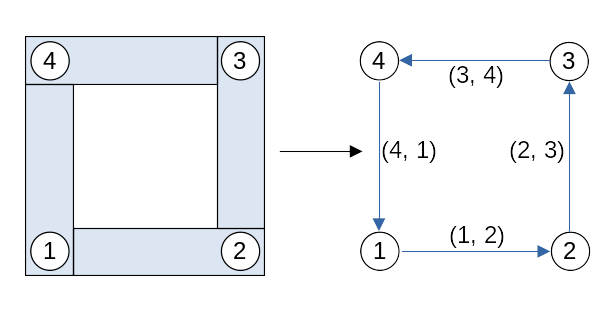
\includegraphics[width=\linewidth]{images/location_encoding.png}
    \caption{Standortenkodierung der Knoten und Pfade.}
    \label{fig:location_encoding}
\end{figure}
\newline
Daraus wird die Komplexität und Genauigkeit dieser Ansätze deutlich.
Der Kantenansatz ist ein Kompromiss zwischen Genauigkeit und Komplexität.
Dabei bestimmt die Anzahl der zu klassifizierenden Standorte die Komplexität.
Zum einen ist gerade bei langen Pfaden eine geringe Auflösung im Vergleich zur Realposition des Objektes zu erwarten,
d. h. es ist unklar, ob sich das Objekt am Anfang, Ende oder in dazwischen befindet.
Zum anderen werden in einem zyklischen Graphen mindestens so viele Standorte, wie beim Knotenansatz verwendet.
Der Knotenansatz benötigt am wenigsten Standorte zur Enkodierung ist aber außerhalb der Standorte sehr ungenau.
Aus einer Historie von vorherigen Standorten kann aber ein möglicher Pfad inferiert werden,
allerdings können auch mehrere Pfade in Frage kommen, z. B. bei einer Gabelung.
Der kombinierte Ansatz enkodiert soviele Standorte wie beide Ansätze zusammen,
wodurch dieser Ansatz am komplexisten ist und am schlechtesten für große Routen skaliert.
Dafür ist die Auflösung des kombinierten Ansatzes so gut, wie eine diskrete Enkodierung es zulässt.
\newline
\newline
Ist in den aufgenommenen Trainingsdaten die Position des Objektes zum Zeitpunkt der Aufnahme der Sensorwerte bekannt,
so können die Standorte nach dem gewählten Enkodierungsansatz beliebig genau beschriftet werden.
Dies kann in einem Weiterverarbeitungsschritt nach der Aufnahme der Daten mit einer Karte von den Interessepunkten geschehen.